\subsubsection{Impressió del gràfic}

\paragraph{}
La funcionalitat evolució temporal d'esdeveniments, utilitza una variable global per comptar quantes iteracions de les enviades al SDK, han estat ja retornades per aquest (\emph{yearsConsulted}).

En el moment en què una petició retorna del SDK i aquesta variable, passa a tenir el valor onze, significa que ja s'han rebut totes les dades i que per tant, aquestes poden ser impreses. Les línies de codi que realitzen la gestió d'aquesta variable, dins de les crides al SDK, es mostren a continuació.

\begin{lstlisting}[style=rawOwn,caption={Gestió de la variable \emph{yearsConsulted}, per controlar el final de la cerca}]
client.getPersonSearch(params).then(function(searchResponse) {
    yearsConsulted = yearsConsulted + 1;
    linechartRows[i].push(String(firstYear+i));
    linechartRows[i].push(total);
    if(yearsConsulted == 11) printLinechart();
});
\end{lstlisting}

Per altra banda, la funcionalitat encarrega d’imprimir el gràfic de línies en el HTML, segueix els mateixos detalls d’implementació, que els mostrats en la funcionalitat evolució geogràfica d’un cognom.

Un exemple del gràfic imprès per aquesta funcionalitat, pot ser vist en la figura~\ref{fig:factsLine}.

\begin{figure}[h]
    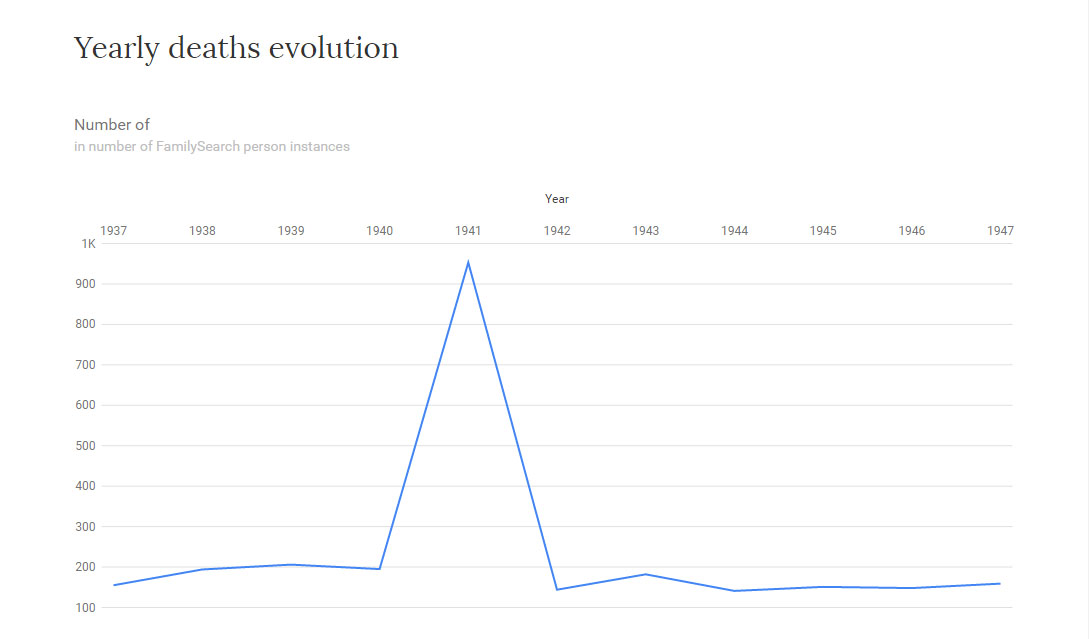
\includegraphics[width=\linewidth]{11/04_factsSearcher/01_yearsEvolution}
    \centering
    \caption{Gràfic de línies de la funcionalitat evolució d'esdeveniments}\label{fig:factsLine}
\end{figure}
